\section{Linux Shell}

	Responda lo siguiente:

		\begin{enumerate}

			\item ¿Quién y en qué año desarrolló el primer shell para UNIX?
			
			Fue creado por Steven R. Bourne, en 1974.
			
			\item ¿Cuál es el nombre del primer shell para UNIX?
			
			Bourne Shell. Nombre adquirido en referencia a su creador. Comúnmente conocido con la abreviatura ''sh''.
			
			Este shell fijó el estándar de shells para UNIX.
			
			Sh permitió un trabajo más simple al realizar tareas repetitivas al introducir los Shell Scripts.
			
			Su modelo de desarrollo se enfocó en la minimización y apertura de uso. Esto conllevó a la dependencia de terceros programas para realizar tareas sencillas, sin embargo, generaba un ambiente de trabajo bastante flexible para el usuario.
			
			\item Mencione tres variantes de shell diferentes a sh
			\begin{itemize}
				\item \textbf{Csh} \newline
				Fue un Shell basado ligeramente en el lenguaje C.
				\item \textbf{Ksh} \newline
				El Korn Shell. Fue una mejora del Bash de Bourne desarrollada por David G. Korn.
				\item \textbf{Bash} \newline
				Acrónimo humorístico de ''Otra vez el Shell de Bourne'' (Bourne Again SHell), el Bash es la mejora directa sobre el Shell de Bourne original. Es retro-compatible, contiene nuevas características y mejoras y acata los estándares POSIX para los Shells.
			\end{itemize}
			
			\item ¿Cuál es el shell en las distribuciones Linux?
			
			Hoy en día, Bash es el shell estándar que viene incluído en casi todas las distribuciones de Linux.
			
			\item ¿Cuál es la extención de un Shell Script?
			
			\textit{.sh}
			
			\item Defina: pathname, relative path y absolute path
			
			\begin{itemize}
			\item \textit{Pathname} \newline
				Es una cadena de carácteres que identifica la ubicación de un archivo particular; la secuencia de directorios a moverse para encontrarlo.
			\item \textit{Relative Path} \newline
				Describe la ubicación de un archivo en relación con el Direcorio Raíz. Se identifica por tener una barra (el mismo Directorio Raíz) al inicio.
			\item \textit{Absolute Path} \newline
				Al contrario de la Relative Path, no inicia con una barra y describe la ubicación de un archivo en relación con el directorio actual.
			\end{itemize}
			
		\end{enumerate}

	Escriba la funci\'on de los siguientes comandos o utilidades: 
			
			\begin{itemize}

				\item man: \newline
				Es una interfaz para los manuales de referencia.
				
				\item cd:\newline
				''Change Directory''. Permite cambiar el directorio activo.
				
				\item cp:\newline
				Permite CoPiar archivos y directorios.
				
				\item mv: \newline
				Permite MoVer y renombrar archivos.
				
				\item ls: \newline
				Permite enLiStar los contenidos del directorio activo.
				
				\item rm: \newline
				Premite ReMover archivos y directorios.
				
				\item pwd: \newline
				Este comando muestra el directorio activo. (Print Working Directory)
				
				\item rmdir: \newline
				Permite remover un directorio vacío. (ReMove DIRectory)
				
				\item mkdir: \newline
				Crea un directorio. (MaKe DIRectory)
				
				\item chmod: \newline
				Cambia los bits del modo de un archivo. Esto controla los permisos del archivo. (CHange MODe)
				
				\item chown: \newline
				Permite cambiar el propietario y grupo de un archivo. (CHange OWNer)
				
				\item touch: \newline
				Permite cambiar el timestamp de un archivo. Si el archivo señalado no existe, se crea vacío.				
				
				\item less: \newline
				Un visor de texto \textit{menos} complejo que ''more'', su antecesor.
				
				\item cat: \newline
				ConCATena archivos y devuelve el resultaro a la salida estándar.
				
				\item sudo: \newline
				Permite ejecutar un comando como otro usuario.
				
				\item su: \newline
				Permite ser el Super-Usuario.
				
				\item apt-get: \newline
				Utilidad que maneja los paquetes APT.
				
				\item clear: \newline
				Limpia la consola.
				
				\item wget: \newline
				Permite descargar en la red de manera no interactiva. (Web GETter)
				
				\item who: \newline
				Muestra quén tiene la sesión activa.
				
				\item whoami: \newline
				Imprime la identidad efectiva del usuario.
				
				\item passwd: \newline
				Permite cambiar la contraseña. (PASSWorD)
				
				\item date:\newline
				Imprime en pantalla la fecha del sistema.
				
				\item uname: \newline
				Imprime la información del sistema.
				
				\item history: \newline
				Presenta el historial de comandos utilizados.
				
				\item tar: \newline
				La versión GNU de la utilidad de compresión TAR.
				
				\item shutdown: \newline
				Permite parar, apagar o reiniciar la máquina.
				Se puede señalar el tiempo deseado para realizar la acción.
				
				\item make:	\newline
				Una herramienta GNU que sirve para mantener grupos de programas.
				
				Concretamente, determina automáticamente que partes de un programa grande necesita ser re-compilado, y genera los comandos para re-compilarlos.
				
				\item printf: \newline
				Función que permite imprimir datos con formato. (PRINT with Format)
				
				\item finger: \newline
				Permiter ver información acerca de los usuarios del sistema.
				
				\item users: \newline
				Permite ver los nombres de los usuarios que están trabajando en el momento.
				
				\item w: \newline
				Permite saber que están haciendo los usuarios activos.
				
				\item alias: \newline
				Permite realizar un conjunto de comandos con una cadena de texto ya definido.

			\end{itemize}

	Escriba en el editor nano/pico el siguiente shell script (Obtenga pantalla):
	
	\begin{flushleft}
		$\sharp$ hello.sh \\
		$\sharp$ This is my first shell script \\
		printf “Hello! Bash is wonderful.” \\
		exit 0
	\end{flushleft}
	\noindent
	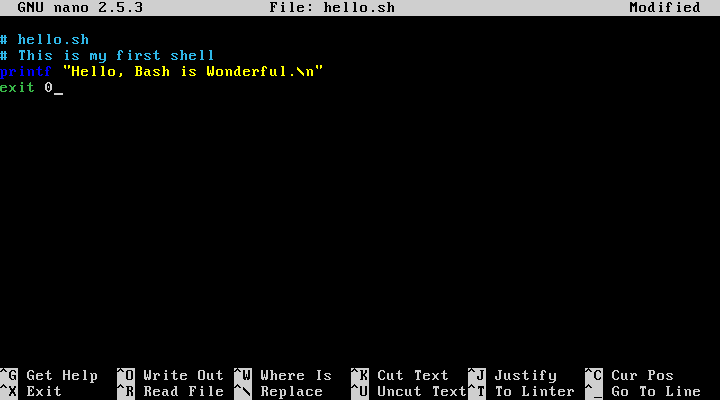
\includegraphics[width=\textwidth]{imagenes/sh.png}

	Guarde el archivo como hello.sh, cambie los modos de acceso para que el dueño y el grupo tengan todos los permisos y los demás ninguno (Obtenga pantalla). \newline
		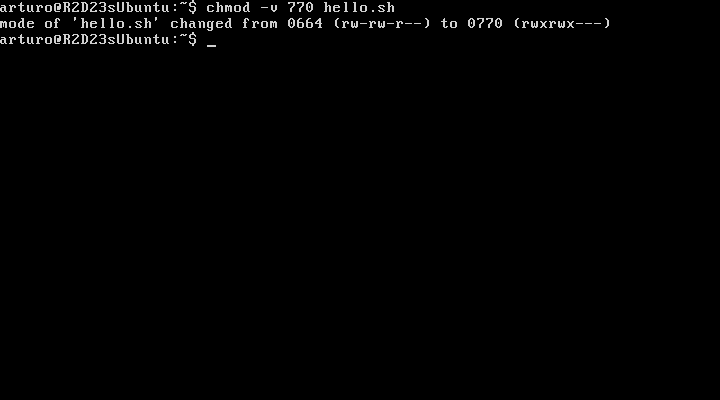
\includegraphics[width=\textwidth]{imagenes/chmod.png}
	A continuación ejecute el shell script con bash y con (Obtenga pantalla de ambas ejecuciones). \newline
		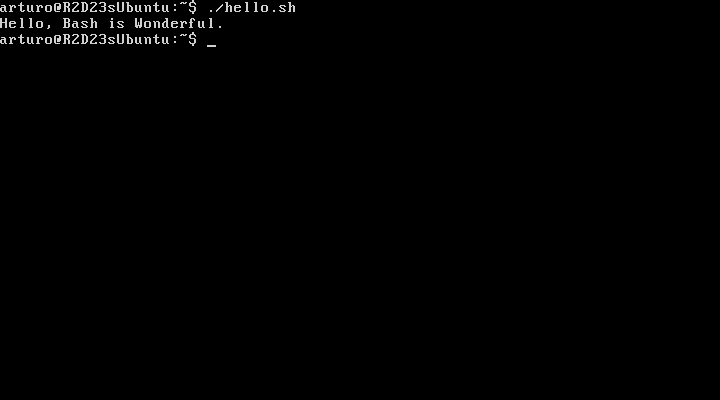
\includegraphics[width=\textwidth]{imagenes/exe.png}